\documentclass[9pt,landscape,a4paper, table]{extarticle}
\usepackage{graphicx}
\graphicspath{ {images/} }
\usepackage{amssymb,amsmath,amsthm,amsfonts}
\usepackage{mathtools}
\usepackage{multicol,multirow}
\usepackage{enumitem}
\usepackage[landscape]{geometry}
\usepackage[explicit]{titlesec}
\usepackage[many]{tcolorbox}
\usepackage{mathrsfs}
\usepackage{fancyhdr}
\usepackage{xcolor}
\usepackage[ruled,linesnumbered]{algorithm2e}

\fancyhf{}
\rfoot{\raisebox{1cm}{Page \thepage}}

\geometry{top=.4cm,left=.5cm,right=.5cm,bottom=.5cm}
\linespread{.5}
\setlist{nosep}

%\pagestyle{fancy}
\setcounter{secnumdepth}{0}

\titleformat{\section}[display]
  {\large\bfseries}{}{0pt}{\begin{tcolorbox}[
      arc=0pt,outer arc=0pt,
      boxsep=0pt,boxrule=0pt,
      left=6pt,right=6pt,top=3pt,bottom=3pt,middle=0pt,
      nobeforeafter,
      colback=cyan!50!blue
      ]\color{white}#1\end{tcolorbox}}
\titleformat{\subsection}[display]
  {\large\bfseries}{}{0pt}{\begin{tcolorbox}[
      arc=0pt,outer arc=0pt,
      boxsep=0pt,boxrule=0pt,
      left=6pt,right=6pt,top=2pt,bottom=2pt,middle=0pt,
      nobeforeafter,
      colback=cyan!20
      ]#1\end{tcolorbox}}
\titleformat{\subsubsection}[display]
  {\normalsize\bfseries}{}{0pt}{\begin{tcolorbox}[
      arc=0pt,outer arc=0pt,
      boxsep=0pt,boxrule=0pt,
      left=6pt,right=6pt,top=2pt,bottom=2pt,middle=0pt,
      nobeforeafter,
      colback=cyan!5
      ]#1\end{tcolorbox}}

\titlespacing{\section}
  {0pt}{5pt}{0pt}
\titlespacing{\subsection}
  {0pt}{0pt}{0pt}
\titlespacing{\subsubsection}
  {0pt}{0pt}{0pt}

\renewcommand{\large}{\normalsize}
%\renewcommand{\normalsize}{\normalsize}
\renewcommand{\small}{\normalsize}

%Setting custom font to FiraSans
\usepackage[utf8]{inputenc}
\usepackage[T1]{fontenc}

\usepackage{mathpazo}
\renewcommand{\rmdefault}{put}

\usepackage{hyperref}
\usepackage[sfdefault]{FiraSans}
%\usepackage{newtxsf}
\usepackage{graphicx}

% Custom math operators
\DeclareMathOperator*{\argmax}{arg\,max}
\DeclareMathOperator*{\argmin}{arg\,min}
\DeclareMathOperator*{\E}{\mathrm{E}}
\DeclareMathOperator*{\Var}{\mathrm{Var}}
\DeclareMathOperator*{\w}{\mathbf{w}}
\DeclareMathOperator*{\W}{\mathbf{W}}
\DeclareMathOperator*{\x}{\mathbf{x}}
\DeclareMathOperator*{\X}{\mathbf{X}}
\DeclareMathOperator*{\y}{\mathbf{y}}
\DeclareMathOperator*{\z}{\mathbf{z}}
\DeclareMathOperator*{\vv}{\mathbf{v}}
\newcommand{\eqqcolon}{\mathrel{\rotatebox[units=360]{180}{\ensuremath{\coloneqq}}}}

% Document

\pagenumbering{gobble}

\begin{document}

\begin{multicols*}{3}
\raggedright

% Title
\large{\textbf{Data Structures and Algorithms} SS20} // \normalsize{Gian Silvan Hiltbrunner}
%\url{https://git.io/JJFdz}

\hrule

% Set lengths
\setlength{\parindent}{0pt}
\setlength{\parskip}{1pt}
\setlength{\abovedisplayskip}{0pt}
\setlength{\belowdisplayskip}{0pt}
\setlength{\abovedisplayshortskip}{0pt}
\setlength{\belowdisplayshortskip}{0pt}

%%%%% Content

\section{Algorithms}

\subsection{Order of Complexity}
\begin{center}
{\footnotesize
$1,\ \log\log n,\ \sqrt{\log n},\ \log\sqrt{n},\ \log n,\ \sqrt{n},\ n,\ n\log n,\ n^2,\binom{n}{3} \in n^3,\ \ n^c,\  2^n,\ n!$
}
\end{center}
{\footnotesize
\begin{align*}
    \lim _{n\rightarrow\infty}\frac{f(n)}{g(n)} = 0 \Rightarrow f \in \mathcal{O}(g), \mathcal{O}(f) \subsetneq \mathcal{O}(g); \lim _{n\rightarrow\infty}\frac{f(n)}{g(n)} = C > 0 (C \text{ constant}) \\ \Rightarrow f \in \Theta (g); \frac{f(n)}{g(n)} \underset{n\rightarrow\infty}{\rightarrow} \infty g \in \mathcal{O}(f), \mathcal{O}(g) \subsetneq \mathcal{O}(f);
    \sum_{k=1}^n k = \frac{n(n+1)}{2}
\end{align*}}

\begin{comment}
\subsection{Maximum Subarray Alogrithm}

{\scriptsize
\begin{algorithm}[H]
    \caption{Inductive Maximum Subarray $\mathcal{O}(n)$}
    
    \SetAlgoLined
    \SetKwInOut{Input}{Input}
    \SetKwInOut{Output}{Output}
    \Input{$(a_1,a_2,..-,a_n)$}
    \Output{$\max{0,\max_{i,j}\sum_{k=i}^j a_k}$}
    \For{$i = 1,..., n$}{
        $R \leftarrow R + a_i$\\
        \If{$R<0$}{
        $R \leftarrow 0$
        }
        \If{$R > M$}{
        $M\leftarrow R$}
    }
    \Return{M}
\end{algorithm}}
\end{comment}

\subsection{Asymptotics of Recursions}

$g: \Theta (2^n)$ $w: \Theta(n\log(n))$ $s: \Theta(n)$
\begin{verbatim}
void g(int n){
    for (int i = 0; i<n ; ++i ){
        g(i)
    } f();
}
void w(int n){
    if (n > 1){ w(n/2); w(n/2); } 
    while (--n > 0){ f(); }
}
void s(int n){ f(); 
if (n>1) { s(n/2); s(n/2); }}
\end{verbatim}


\section{Searching}

\subsection{Linear Search}

Best case: 1 comparison; 
Worst case: n comparisons\\
Expected: $\mathrm{E}(x) = \frac{1}{n}\sum_{i=1}^n i = \frac{n+1}{2} \in \Theta(n)$

\subsection{Binary Search}
divide and conquer approach $\rightarrow \Theta(\log n)$
Works with two pointers $l$ and $r$. If $l > r$ the search was without result.

{\scriptsize
\begin{algorithm}[H]
    \caption{Breadth-first search}
    
    \SetAlgoLined
    \SetKwInOut{Input}{Input}
    \SetKwInOut{Output}{Output}
    \Input{A graph G and a starting vertex root of G}
    \Output{The parent links trace the shortest path back to root}
    let Q be a queue; label root as discovered; Q.enqueue(root)\\
    \While {Q is not empty}{
           v := Q.dequeue()
           \If {v is the goal}{
                \Return v
           }
           \For {all edges from v to w in G.adjacentEdges(v)}{
             \If {w is not labeled as discovered}{
            label w as discovered\\
            w.parent := v; Q.enqueue(w)
             }
           }
    }
\end{algorithm}}

\section{Selecting}

\subsection{Blum's Algorithm}
A good pivot can be selected using the median-of-medians-algorithm. $\mathcal{O}(n)$

\begin{enumerate}
    \item Consider groups of 5 elements
    \item Compute the median for each group (trivial)
    \item Recursively compute medians
\end{enumerate}

\subsection{Pivot}
{\scriptsize
\begin{algorithm}[H]
    \caption{Selection via Pivot}
    
    \SetAlgoLined
    \SetKwInOut{Input}{Input}
    \SetKwInOut{Output}{Output}
    \Input{Array A of length n with pivot p}
    \Output{A partitioned around p with position of p}
    $l \leftarrow 1$\\
    $r \leftarrow n$
    \While{$l \leq r$}{
        \While{$A[l] < p$}{
        $l \leftarrow l + 1$
        }
        \While{$A[r] > p$}{
        $r \leftarrow r -1$
        }
        swap(A[l],A[r])
        \If{$A[l] = A[r]$}{
        $l \leftarrow l + 1$}
    }
    \Return{$l-1$}
\end{algorithm}}

{\scriptsize
\begin{algorithm}[H]
    \caption{Quickselect $\mathcal{O}(n)$}
    
    \SetAlgoLined
    \SetKwInOut{Input}{Input}
    \SetKwInOut{Output}{Output}
    \Input{Array A of length n; $1 \leq k \leq n$}
    %\Output{Product $x\cdot y$}
    $x \leftarrow$ RandomPivot(A)\\
    $m \leftarrow$ Partition(A,x)\\
    \If{$k<m$}{
    \Return{Quickselect(A[0..m-1],k)}
    }
    \If{k > m}{
    \Return{Quickselect(A[m+1..n],k)}
    \Else{\Return{$A[k]$}}
    }
\end{algorithm}}

\section{Sorting}

%\begin{center}
%   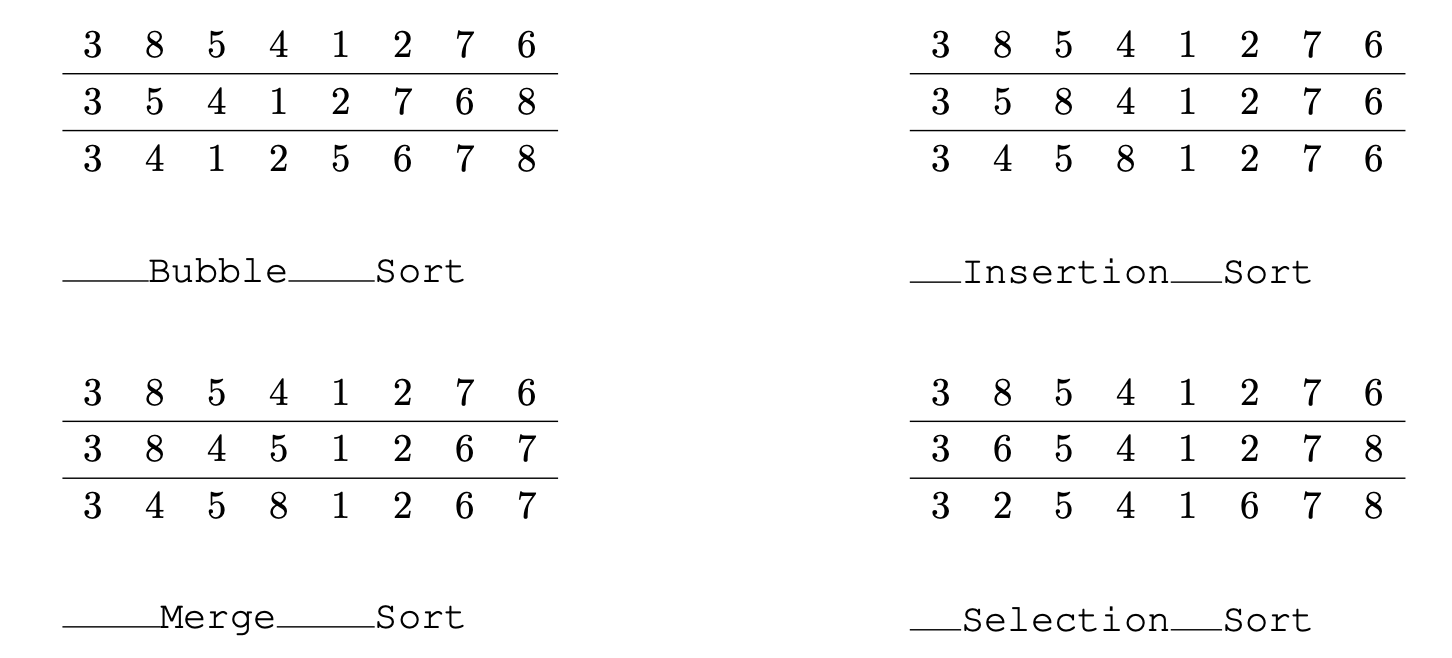
\includegraphics[width = 1\linewidth]{img/Sorting.png}
%\end{center}
%We should think about how to do the sorting algorithms
\begin{itemize}
    \item \textbf{Bubblesort}: Swap if $A[i-1]> A[i]$. In each round, the max in the unsorted part will move to the right. $\Theta(n^2)$ stable
    \item \textbf{Selection sort}: swap the smallest element in the unsorted part with the most right element of the sorted part. $\Theta(n^2)$ unstable
    
    \begin{verbatim}
arr[] = 64 25 12 22 11
// Place min at beginning
11 25 12 22 64
// Place min at beginning
11 12 25 22 64 ...
    \end{verbatim}
    
    \item \textbf{Insertion sort}: Determine the insertion position of element i. $\Theta(n^2)$ stable
    
\begin{verbatim}
1: Iterate over the array (curr).
2: Compare curr to predecessor (pre).
3: If curr < pre,
compare it to the elements before.
Larger elements are moved back 1 pos.
\end{verbatim}
    \item \textbf{Merge sort}: At least two parts of the Array are already sorted. Iterative merging of the already sorted bits. - $\Theta(n \log n)$,  $\Theta(n)$ storage, stable,  needs intermediate storage for the merging step

\item \textbf{Quicksort}
1. Pick a pivot 2. Partitioning: reorder the array so that all elements with values less than the pivot come before the pivot, while all elements with values greater than the pivot come after it (equal values can go either way). After this partitioning, the pivot is in its final position. 3. Recursively apply the above steps to the sub-array of elements with smaller values and separately to the sub-array of elements with greater values.
\end{itemize}



\subsection{Quicksort}
{\scriptsize
\begin{algorithm}[H]
    \caption{Quicksort $\mathcal{O}(n\cdot \log n)$}
    
    \SetAlgoLined
    \SetKwInOut{Input}{Input}
    \SetKwInOut{Output}{Output}
    \Input{Array A of length n}
    \Output{Array A sorted}
    \If{$n>1$}{
    Choose Pivot $p \in A$
    $k \leftarrow$ Partition(A,p)\\
    Quicksort(A[1,...,k-1])\\
    Quicksort(A[k+1,...,n])
    }
\end{algorithm}}

{\scriptsize
\begin{algorithm}[H]
    \caption{Partition}
    
    \SetAlgoLined
    \SetKwInOut{Input}{Input}
    \SetKwInOut{Output}{Output}
    \Input{Array A, that contains the pivot p in A[l, . . . , r] at least once.}
    \Output{Array A partitioned in [l, . . . , r] around p. Returns position of p.}
    
    \While {$l \leq r$}{
    \While {$A[l] < p$}{
        $l=l+1$
    } 
    \While {$A[r] > p$}{
        $r=r-1$
    } 
    swap($A[l], A[r]$)
    
    \If {$A[l] = A[r]$}{
        $l=l+1$ 
    }
    }
    return $l-1$
\end{algorithm}}

Runtime: ${\Theta}(n\cdot \log n)$, worst case $\Theta(n^2)$ if worst pivots are selected each time.

\subsection{Radix Sort}
n-locks for n-keys $\in \mathcal{O}(n)$. We have m-adic binary numbers, so two categories to sort the numbers into. Used for numbers (and strings via UTF-8/ASCii)
\subsection{Bucket Sort}
Create a number of buckets. Sort e.g. after decimality into buckets and sort those buckets then. Can be implemented via linked list.


\begin{center}
    \hspace{1cm}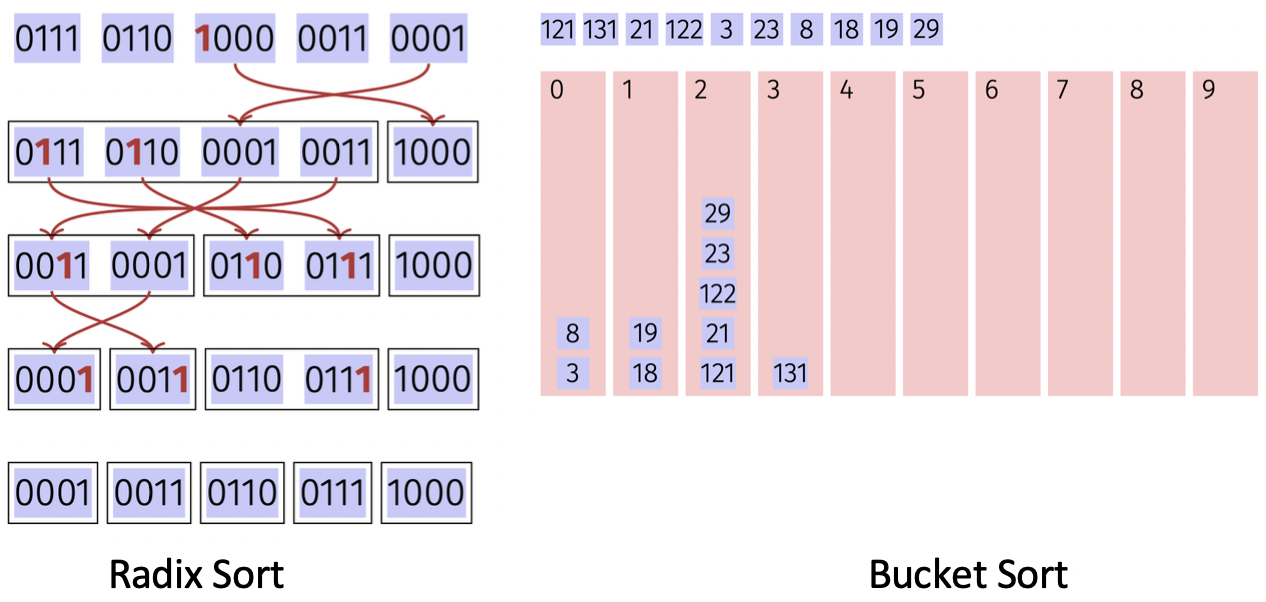
\includegraphics[width = 0.6\linewidth]{img/Bucket.png}
\end{center}



\section{Hashing}

\subsection{Basics}
Common: $h(k) = k \mod m$\\
Often: $m = 2^k - 1$\\

\textbf{Linear Probing}: $S(k) = (h(k), h(k) + 1 ,..., h(k) + m - 1)\mod m$
\textit{Issue}: Primary clustering, long contiguous areas of used entries.\\ 
\textbf{Quadratic Probing}: $S(k) = (h(k), h(k) + 1, h(k) -1, h(k) + 4, ...)\mod m$ \textit{Issue}: Secondary clustering, traversal of the same probing sequence.\\ 
\textbf{Double Hashing}: $S(k) = (h(k),h(k)+h'(k),h(k)+2h'(k),...,h(k)+(m-1)h'(k))\mod m$

\section{Trees}
Trees are connected, directional and acyclic graphs.

\subsection{Removing a child}
\begin{itemize}
    \item No children - Remove the node
    \item 1 child - Replace by the only child
    \item 2 children - Replace by the symmetric descendent
\end{itemize}

\subsection{Ways of traversal}
\subsubsection{Preorder}
$v$, then $T_{left}(v)$, next $T_{right}(v)$
\subsubsection{Postorder}
$T_{left}$, then $T_{right}$, next $v$
\subsubsection{Inorder}
$T_{left}$, then $v$, next $T_{left}$ $\rightarrow$ ascending sequence.

\subsection{Heaps}
Keys are strictly larger/smaller depending on Max- or Minheap. If the root is at index $0$: Children at indices $2i + 1$ and $2i + 2$
\subsubsection{Build}
In order to build a heap we run \texttt{heapify} on each element letting it trickle down. This takes $n\cdot \log n$ steps. Thus we get a runtime of $\mathcal{O}(n \log n)$ 
\subsubsection{Insertion}
Inserting a key into a heap can possibly violate the heap settings - Is reinstated by successive rising up. 
\subsubsection{Heap Sort}
Non-stable sort using inductive sorting from below. With a running time of $\mathcal{O}(n\cdot \log n)$.

\begin{enumerate}
    \item Call the buildMaxHeap() function on the list. Also referred to as heapify(), this builds a heap from a list in O(n) operations.
\item Swap the first element of the list with the final element. Decrease the considered range of the list by one.
\item Call the siftDown() function on the list to sift the new first element to its appropriate index in the heap.
\item Go to step (2) unless the considered range of the list is one element.
\end{enumerate}

\subsection{Quadtrees}
Partitioning a subsection into 4 equal parts. If there are too many objects stored in one node, we split the node into four children. Objects that are falling on a border are stored in the parent node.

\subsection{AVL trees}
AVL trees guarantee a runtime of $\mathcal{O}(\log n)$\\
$bal (v) \coloneqq h(T_r(v))-h(T_l(v))$\\
AVL condition: $\forall v \in V: bal(v) \in \{-1,0,1\}$

\subsubsection{Rebalancing AVL trees}
{
\hspace{1cm}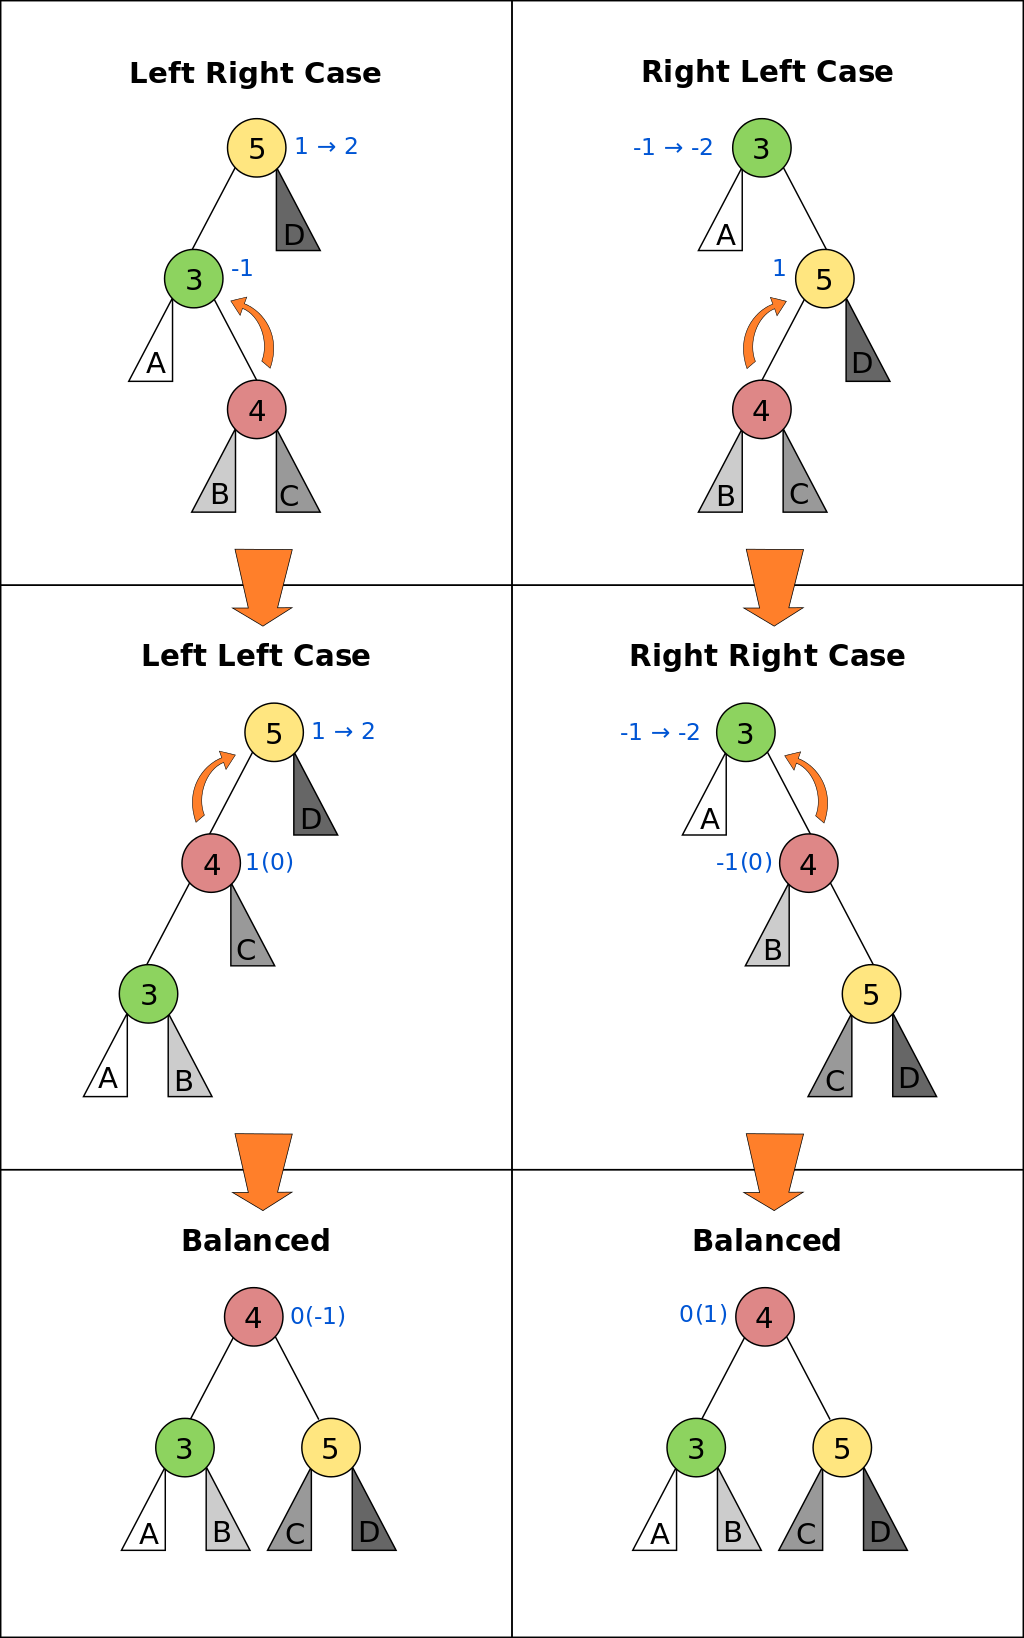
\includegraphics[angle=90,width = 1\linewidth]{img/AVL_Tree_Rebalancing.png}
}

\section{Dynamic Programming}

\subsection{Samples}

\textbf{One-dimensional}\\
\textit{Problem}: Finding the longest possible combination of downwards ski slopes with lengths $l_i$. The slopes connect the stations with heights $h_i$.  
\begin{enumerate}
    \item \textbf{Table}: $n\times 1$ 
    \item \textbf{Entry}: $[i]$: longest descent that ends in $i$.
    \item \textbf{Calculation}: $D[i] = 0, \forall i = 1, ... ,n$ and $\displaystyle D[i] = \max_{Slope(j,i)}\{D[j] + l(j,i)\}$
    \item \textbf{Order}: \texttt{for i in (1, n); D[i]}
    \item \textbf{Result}: $\max(D)$
    \item \textbf{Reconstruction}: Recursively walk back from result and check $\displaystyle D[i] = D[j] + l(j,i)$ for all slopes $(j,i)$
\end{enumerate}

\textbf{Two-dimensional}\\
\textit{Problem}: Finding the smallest possible value of an expression ($n$ values $a_i$ and $n-1$ operators $s_i$) using optimal bracket placement. 
\begin{enumerate}
    \item \textbf{Table}: $n\times n$: Only upper right triangular matrix is used. 
    \item \textbf{Entry}: $[i,j]$: smallest possible value of sub-expression from value $a_i$ to $a_j$.
    \item \textbf{Calculation}: $A_{i,i} = a_i; 1\leq i \leq n$ and $\displaystyle A_{i,j} = \min_{i\leq k \leq j}\{A_{i,k-1}\langle s_{k-1}\rangle A_{k,j}\}; 1\leq i\leq j\leq n$
    \item \textbf{Order}: \texttt{for s in (0, n-1); for i in (1, n-s); A[i,i+s]}
    \item \textbf{Result}: \texttt{A[1,n]}
    \item \textbf{Reconstruction}: Recursively walk back and check $\displaystyle A_{i,j} = A_{i,k-1}\langle s_{k-1}\rangle A_{k,j}$
\end{enumerate}

%\subsection{Classes of Problems}



\section{Graphs}

\subsection{Basics}

\textbf{Connected}: Graph where there is a connecting path (not edge) between each pair of nodes.\\
\textbf{Complete}: Graph where there is an edge between each pair of nodes. 



{\scriptsize
\begin{algorithm}[H]
    \caption{Depth First Search}
    
    \SetAlgoLined
    \SetKwInOut{Input}{Input}
    \SetKwInOut{Output}{Output}
    \Input{A graph G and a vertex v of G}
    \Output{All vertices reachable from v labeled as discovered}
    label v as discovered\\
    \For {E $\in$ G.adjacentEdges(v) (lexicographic)}{
            \If{vertex w is not labeled as discovered}{DFS(G, w)}
    }

\end{algorithm}}

\section{Topological Sorting} {
A directed graph has a topological sorting if it is acyclic. \textbf{Idea} We successively prune our graph by removing elements that have 0 entry edges (and then update the entry edges of the successors to find the next one.

{\scriptsize
\begin{algorithm}[H]
    \caption{Topological Sorting}
    
    \SetAlgoLined
    \SetKwInOut{Input}{Input}
    \SetKwInOut{Output}{Output}

$A[v]$ contains number of entry edges of vertex v (calculate by setting $A[w] = 0$ and then loop through $(v, w) \in E$ and set $A[w] += 1$ 

\For{$v \in V$ where $A[v] == 0$}{Push($S$, $v$)}
i=0;

\While{$S != \{\} $  }{
	$v \leftarrow $ pop($S$);
	ord[$v$] $ \leftarrow  i $
	
	$i$++;
	
	\For{ (v, w) in E }{
	
		$A[w] \leftarrow A[w] - 1$ ; //decrease incoming for all successors
		
		\If{A[$w$] == 0}{push($S$,$w$)} 
	}
}
\If{i = |V|}{return SUCCESS}
\Else{ return “Cycle detected” }
\end{algorithm}
}

}

\section{Shortest Path}
On either directed or non-directed, weighted graph, find the shortest distance between a point A and all the other points in the graph.

\subsection{Dijkstra}

{\scriptsize
\begin{algorithm}[H]
    \caption{Dijkstra $\mathcal{O}(|E|  log |V|) $}
    
    \SetAlgoLined
    \SetKwInOut{Input}{Input}
    \SetKwInOut{Output}{Output}
    \Input{$G = (V,E, source)$}
    %\Output{Product $x\cdot y$}
    create vertex set Q //as a queue / min heap;
    
    \For{$u \in V$}{
        $dist[u] \leftarrow$ INFINITY;
        
        $prev[u] \leftarrow$ UNDEFINED;
        
        $Q.insert(u);$
    
    }
    $dist[source] =$ 0;
    

    \While{$Q$ not empty}{
        $u = Q.ExtractMin()$;
        
        \For{$v$ in Neighbors of $u$ still in $Q$}{
            $alt =  dist[u] + length(u,v)$;
            
            \If{$alt < dist[v]$}
            {  
                $dist[v] = alt$;
                
                $prev[v] = u$;
                
                $Q$.DecreasePriority($v, alt$);
            }
        }
    }
\end{algorithm}}

\begin{itemize}
    \item Any data structure: $\mathcal{O}(|V|\cdot T_{em} + |E| \cdot T_{dp})$
    \item With an array or linked list $\mathcal{O}(|V|^2 + |E|) = \mathcal{O}(|V|^2) $
    \item Dense graph in adjacency list $\mathcal{O}(|V|^2 log |V|) $ since $|E| = |V|^2$ and DecreaseKey $log(|V|)$
    \item Sparse connected graph in adjacency list/ stored in binary tree $\mathcal{O}(|E|  log |V|) $
\end{itemize}

\subsection{A-Star}

$A^*$ is an extension of Dijkstra's algorithm using a additional heuristic to guide the direction of the search. Like Dijkstra, A* works by making a lowest-cost path tree from the start node to the target node but it uses a function $f(n)$ as an estimate of the total cost using this path. 

$$f(n) = g(n) + h(n)$$

$f(n)$ :total estimated cost of path through node $n$,
$g(n)$: cost so far to reach node $n$,
$h(n)$: estimated cost from $n$ to goal.\\

A good heuristic $h(n)$ is the Manhattan distance. 

\subsection{Bellman-Ford}

Instead of optimizing the order in which vertices are processed, Bellman-Ford simply relaxes all the edges $|V| - 1$ times and hence runs in $\mathcal{O}(|V| |E|)$ time.\\
If we want to limit the number of edges that we pass trough for our solution we can limit the outer loop to only run $k - 1$ times.

{\scriptsize
\begin{algorithm}[H]
    \caption{Bellman-Ford $\mathcal{O}(|E| \cdot |V|) $}
    
    \SetAlgoLined
    \SetKwInOut{Input}{Input}
    \SetKwInOut{Output}{Output}
    \Input{$G = (V,E, source)$}
    
    \For{$u \in V$}{
        $dist[u] \leftarrow$ INFINITY;
        
        $prev[u] \leftarrow$ UNDEFINED;
    
    }
    $dist[source] =$ 0;
    

    \For{$u$ in $|V|$}{
        
        \For{$v$ in Neighbors of $u$}{
            $alt =  dist[u] + length(u,v)$;
            
            \If{$alt < dist[v]$}
            {  
                $dist[v] = alt$;
                
                $prev[v] = u$;
            }
        }
    }
    
    \For{each edge ($u$, $v$) with weight $w$ in $|E|$}
    {
        \If{$dist[u] + w < dist[v]$}
        {
            error "Graph contains a negative-weight cycle"
        }
    }
\end{algorithm}}




\subsection{Floyd-Warshall}

Goal is to find the shortest path between all pairwise edges in a Graph G.

{\scriptsize
\begin{algorithm}[H]
    \caption{Floyd-Warshall $\mathcal{O}(|V|^3) $}
    
    \SetAlgoLined
    \SetKwInOut{Input}{Input}
    \SetKwInOut{Output}{Output}
    \Input{$G = (V,E)$}
    
    
    let $G$ dist be a $|V| × |V|$ array of minimum distances initialized to $\infty$
    
    
\For{each edge ($u$, $v$)} 
{
    dist[$u$][$v$] $\leftarrow$ $w(u, v)$  // The weight of the edge (u, v)
}

\For{each vertex $v$}
{
    dist[v][v] $\leftarrow$ 0
}

\For{k from 1 to $|V|$}
{
    \For{i from 1 to $|V|$} {
        \For{j from 1 to $|V|$} { 
            \If{dist[i][j] > dist[i][k] + dist[k][j]} { 
                dist[i][j] $\leftarrow$ dist[i][k] + dist[k][j];
                
            }
        }
    }
}
\end{algorithm}}



\subsection{Johnson's Algorithm}

\begin{center}
    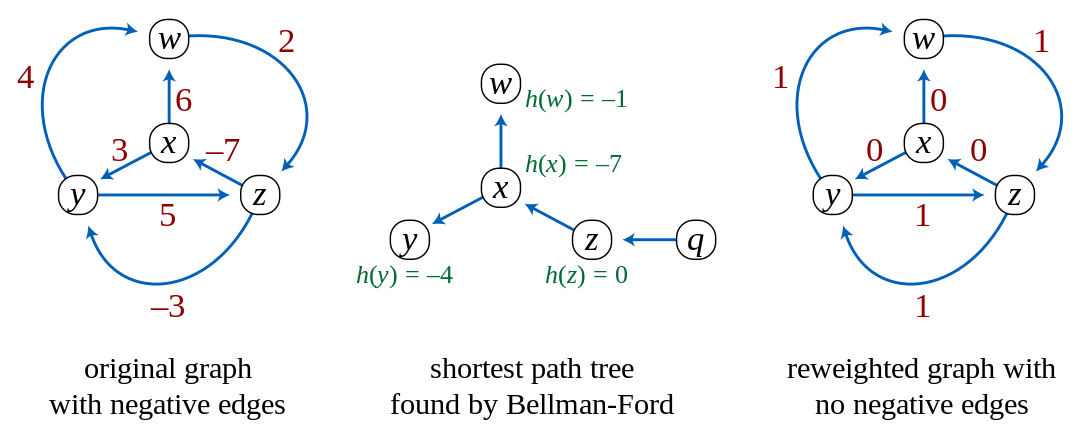
\includegraphics[width=0.7\linewidth]{img/johnson.png}
\end{center}
\vspace{-0.2cm}

Find the shortest paths between all pairs of vertices in an edge-weighted (negative), directed graph. Negative cycles are not allowed. It uses Bellman-Ford to remove all negative weights and then applies Dijkstra on the graph. The runtime is given by $\mathcal{O}(|V|^{2}\log |V|+|V||E|)$. Thus when the graph is sparse the algorithm is faster than Floyd-Warshall which solves the same problem in $\mathcal{O}(|V|
^3)$. 

\begin{enumerate}
    \item New node $q$ is added to the graph connected by zero-weight edges to each of the other nodes. 
    \item Bellman-Ford is used starting from the new vertex $q$ to find the minimum weight from $q$ to each vertex $v$. If a negative cycle is detected the algorithm terminates. 
    \item The original edges are reweighted using the values computed in the Bellman-Ford step. $w'(u,v) = w(u,v) + h(u) - h(v)$
    \item $q$ is removed and Dijkstra is used to find the shortest paths from each node $s$ to every other vertex in the reweighted graph. The original distance is computed by adding $h(v)- h(u)$.
\end{enumerate}

\subsection{Choice of algorithm}
\begin{itemize}
	\item No weights or all equal weights $\rightarrow$ BFS ($\Theta(|V|+|E|)$)
	\item Only positive weights $\rightarrow$ Dijkstra with Fibonacci Heap ($\mathcal{O}(|V|\cdot \log(|V|) + |E|)$)
	\item Some negative weights $\rightarrow$ Bellman Ford ($\mathcal{O}(|E|\cdot|V|^2)$)
	\item All pairs of shortest paths.
	\begin{itemize}
	    \item V times Dijkstra. If negative edges, recreate graph with Johnson first $\mathcal{O}(|E| \cdot |V|  log |V| )$
	    \item Floyd-Warshall. $\mathcal{O}( |V|^3 )$
	    \item Johnsons on a sparse graph. $\mathcal{O}(|V|^{2}\log |V|+|V||E|)$
	\end{itemize} 
	
\end{itemize}

\section{Minimum Spanning Tree}
Given is a undirected weighted connected graph $G(V,E)$. Searched is a minimum spanning tree:
\begin{itemize}
    \item Tree: connected and acyclic
    \item Spanning tree: All vertices $v \in V$ are connected.
    \item minimal: $c(T) = \min \sum_{e \in E} c(e)$
\end{itemize}
\subsection{Kruskal algorithm}

{\scriptsize
\begin{algorithm}[H]
    \caption{Kruskal $\mathcal{O}(E \log E)$}
    
    \SetAlgoLined
    \SetKwInOut{Input}{Input}
    \SetKwInOut{Output}{Output}
    %\Input{$(a_1,a_2,..-,a_n)$}
    %\Output{$\max{0,\max_{i,j}\sum_{k=i}^j a_k}$}
    Sort edges increasingly after their weight:
    $c(e_1) \leq c(e_2) \leq... c(e_m)$\\
    $A \leftarrow \emptyset$
    \For{k = 1 to m}{
        \If{$A \cup {e_k}$}{
            $A \leftarrow A \cup {e_k}$
        }
    }
\end{algorithm}}
Starts with the smallest edge! Edges that would create a cycle are subsequently discarded in the process $\rightarrow$ exam question.\\

\subsection{Jarnik (Prims) Algorithm}
{\scriptsize
\begin{algorithm}[H]
    \caption{Jarnik Algorithm $\mathcal{O}(E + V \log V)$}
    
    \SetAlgoLined
    \SetKwInOut{Input}{Input}
    \SetKwInOut{Output}{Output}
    start with $v \in V$
    $A \leftarrow \emptyset$\\
    $S \leftarrow {v_0}$
    \For{i = 1 to |V|}{
    choose cheapest $(u,v)$ with $u \in S$ and $v \notin S$\\
    $A \leftarrow A \cup {(u,v)}$\\
    $S \leftarrow S \cup {v} $
    }
\end{algorithm}}
Main difference to Kruskal is, that it starts at $v \in V$ and chooses the cheapest edge from there.\\
Runtime: $\mathcal{O}(E + V \log V)$ with fibonacci heaps.
\subsection{\texttt{UnionFind}}
Find(x): Find the node x, go to the root of this subtree and return it.
Union: Add the smaller subtree as a child to the larger subtree.

\section{Max Flow / Min Cut}
Given a flow network, determine the maximal flow allowed.
The cut of the Graph G(S,T) into a source graph S and a sink graph T with the smallest capacity (min cut) will have the same capacity as the maximal flow.

\subsection{Ford-Fulkerson}

{\scriptsize
\begin{algorithm}[H]
    \caption{Ford-Fulkerson}
    
    \SetAlgoLined
    \SetKwInOut{Input}{Input}
    \SetKwInOut{Output}{Output}
    
    \For{$(u,v) \in E$}{
        $f(u,v) = 0$;
    }
    //$G_f$ describes network capacities minus the existing flows
    
    \While{ Path $p$ exists from s to t in residual network $G_f$ }
    {
        $c_f(p) \leftarrow min( c_f(u,v)  \in p )$;
        
        //increase the flow along this path
        
        \For{ edge $e(u,v) \in p$ } {
            $f(e) \leftarrow f(e) + c_f(p)$;
            
            $c_f(e) \leftarrow c_f(e) - c_f(p)$;
            
        }
    }
\end{algorithm}}

\subsection{Edmonds-Karp}
Edmonds-Karp implements the Ford-Fulkerson algorithm by using a BFS search on the residual network.

\textbf{Runtime of Ford-Fulkerson with Integers}
If $f*$ is the maximum flow in the graph then,
$\mathcal{O}(|E| \cdot f*)$, because the flow needs to increase by at least 1 in each iteration and each can be done in $\mathcal{O}(|E|)$ time. 

\textbf{Runtime of Edmonds-Karp}
$\mathcal{O}(|V||E|)$ iterations, each of which can be done in $\mathcal{O}( |E|)$ times, so $\mathcal{O}(|V||E|^2)$

\subsection{Classes of Problems}

\textbf{Shortest-Path Problem}
\begin{itemize}
    \item Representation of simple graph with nodes representing the actual states (e.g. city).
    \item Representation of state space with nodes representing the current state of the system. (e.g. city and money left) $\rightarrow$ City is connected to neighbouring cities with the states that the system can take from here. ($A_{5\$}$ $\underset{-2\$}{\rightarrow}$ $B_{3\$}$)
    \item Finding a shortest path of length exactly $l$. We use a layered graph with $l$ layers. Then we run Dijkstra on this graph. (Finding the shortest path when visiting $l$ cities.)
    \item Cycle detection problem - e.g. figuring out if we can generate $\infty$ revenue. The check includes if the shortest path to node 1 has decreased after one more iteration of the outermost loop of Bellman-Ford. The Bellman–Ford algorithm will converge after iterating through the edges at most $| V | -1$ times (as there cannot be more edges in a shortest path) if and only if there is no such negative cycle.
\end{itemize}

\textbf{Bipartite Matching Problem}
\begin{itemize}
    \item Two classes of nodes that need to be matched in an optimal fashion. Use either Ford-Fulkerson or Edmonds-Karp depending on the runtime. 
\end{itemize}

\textbf{Minimum Spanning Tree Problem}

\begin{itemize}
    \item Finding the minimal tree to connect all nodes of a tree/subtree. Use Kruskal or Prim for a dense graph. 
\end{itemize}

\textbf{Failure Resilience Problem}

\begin{itemize}
    \item Edge disjoint graph - Maximal flow $- 1$ between A and B gives the number of edges that can be removed before the connection fails. 
    \item Node disjoint graph - Replace each node with an edge - Model failure state by this edge weight. 
\end{itemize}

\section{Parallel Programming}
Amdahl assumes a fixed relative sequential portion ($\lambda$), Gustafson assumes a fixed absolute sequential part.

\textbf{Amdahl}: $S_A = \frac{1}{\lambda + \frac{1-\lambda}{p}}$\ \textbf{Gustafson}: $S_G=p-\lambda(p-1)$

\subsection{Speedup Calculation}
$T_p \leq \frac{T_1}{p} + T_\infty $ $^*$ |  $S_p = \frac{T_1}{T_p}$\\
$T_{\infty} = $ longest single path | $S_{\infty} = \frac{T_1}{T_{\infty}}$

In order to comply with the estimates for a greedy scheduler, it must hold that $*$ and the \textbf{Lower Bound Laws} hold. 
\subsection{Performance Model}

We have $p$ processors and the corresponding execution time $T_p$.
$T_{\infty}$: The span of the execution network or longest path. Thus the time needed if we have an infinite number of processors. 

$$\text{Parallelism} = T_1/T_\infty$$\\

\textbf{Lower Bound Laws}

\begin{align*}
    T_p \geq T_1/p\quad \text{Work law}
    \qquad T_p \geq T_\infty\quad \text{Span law}
\end{align*}

\textbf{Work and Span for Recursions}

$$T_1(n) = r\times T_1(n_{new}) + \Theta,\ T_\infty(n) = T_\infty(n_{new}) + \Theta$$

If the setup is not fully concurrent then $T_\infty$ will depend on the maximal concurrency. For four recursive calls which are joined as groups of two we have: $\Theta(2^{\log_4(n)}) = \Theta(n^{\log_4(2)}) = \Theta(n^{\frac{1}{2}})$

\subsection{Parallel Programming in C++}

\subsubsection{\texttt{std::mutex}}
\begin{itemize}
    \item Owned when \texttt{lock} was called until \texttt{unlock} is called. 
    \item When owned all other threads block (halt) when \texttt{lock} is called. 
\end{itemize}

\subsubsection{\texttt{std::unique\_lock}}

\begin{verbatim}
    std::unique_lock<std::mutex> lck (mtx);//Locked
    lck.unlock();
\end{verbatim}

\begin{itemize}
    \item In locked state upon construction unless deferred using \texttt{std::defer\_lock}.
    \item Will handle unlocking upon destruction like \texttt{std::lock\_guard} but additionally provided locking and unlocking capabilities. 
\end{itemize}

\subsubsection{\texttt{std::condition\_variable}}

\begin{verbatim}
    std::condition_variable cv;
    std::unique_lock<std::mutex> lk(m);
    cv.wait(lk, []{return x == 1;});
    
    lk.unlock();
    cv.notify_one();
    cv.notify_all();
\end{verbatim}


\begin{itemize}
    \item \texttt{std::condition\_variable} takes a \texttt{std::unique\_lock<std::mutex>} which protects the shared variable.
    \item Releases the \texttt{std::mutex} and executes a wait operation on the current thread if the condition does not hold. 
    \item Upon \texttt{notify\_all} or \texttt{notify\_one} wakeup it will reacquire the mutex atomically and check the condition. 
\end{itemize}

\subsubsection{Examples}
\textbf{Readers-Writers Lock}
\begin{verbatim}
void acquire_read(){
    guard lock(m);
    c.wait(lock,[&]{return number_writers == 0 ;});
    ++number_readers;
}
  
void release_read(){
    guard lock(m);
    assert(number_readers > 0);
    --number_readers;
    if (number_readers == 0){
      c.notify_all();
    }
}
\end{verbatim}
\textbf{Reentrant Lock}
\begin{verbatim}
void lock(){
    std::thread::id current = std::this_thread::get_id();
    guard lck(m);
    cv.wait(lck, [&]{return count == 0 or id == current;});
    if (id != current) id = current; 
    count++;
}

void unlock(){
    guard lck(m);
    count--;
    if (count == 0) cv.notify_one();
}
\end{verbatim}

\subsection{Race Conditions}
\subsubsection{Data Race}
Bad synchronisation of a shared resource, e.g. two writing processes at the same time.
\subsubsection{Bad Interleaving}
Unlucky order of execution of e.g. two threads even though the shared resource is otherwise well synchronised.

\section{Complexities}

{

\setlength\tabcolsep{3pt}
\begingroup
\footnotesize
\renewcommand{\arraystretch}{2} 
\begin{tabular}{|c | c c c | c|}
    \hline
        \textbf{Algorithm} &  \multicolumn{3}{c|}{Time Complexity}   & Space Complexity \\
         & Best & Average & Worst & Worst \\ \hline
        Quicksort & \cellcolor{orange} $\Omega(n\cdot log(n))$ & \cellcolor{orange} $\Theta(n \cdot log(n))$ & \cellcolor{red} $\mathcal{O}(n^2)$ & \cellcolor[HTML]{9acd32} $\mathcal{O}(log(n))$ \\ \hline
        Mergesort & \cellcolor{orange} $\Omega(n \cdot log(n))$ & \cellcolor{orange} $\Theta (n \cdot log(n))$ & \cellcolor{orange} $\mathcal{O}(n \cdot log(n))$ & \cellcolor{yellow} $\mathcal{O}(n)$ \\ \hline
        Heapsort & \cellcolor{orange} $\Omega(n\cdot log(n))$ & \cellcolor{orange} $\Theta(n \cdot log(n))$ & \cellcolor{orange} $\mathcal{O}(n \cdot log(n))$ & \cellcolor{green} $\mathcal{O}(1)$ \\ \hline
        Bubble Sort & \cellcolor{yellow} $\Omega(n)$ & \cellcolor{red} $\Theta(n^2)$ & \cellcolor{red} $\mathcal{O}(n^2)$ & \cellcolor{green} $\mathcal{O}(1)$ \\ \hline
        Insertion Sort & \cellcolor{yellow} $\Omega(n)$ & \cellcolor{red} $\Theta(n^2)$ & \cellcolor{red} $\mathcal{O}(n^2)$ & \cellcolor{green} $\mathcal{O}(1)$ \\ \hline
        Selection Sort & \cellcolor{red}$\Omega(n^2)$ & \cellcolor{red} $\Theta(n^2)$ & \cellcolor{red} $\mathcal{O}(n^2)$ & \cellcolor{green} $\mathcal{O}(1)$ \\ \hline
        Shell Sort & \cellcolor{orange} $\Omega(n\cdot log(n))$ & \cellcolor{red} $\Theta(n \cdot log(n)^2)$ & \cellcolor{red} $\mathcal{O}(n \cdot log(n)^2)$ & \cellcolor{green} $\mathcal{O}(1)$ \\ \hline
        Bucket Sort & \cellcolor{green} $\Omega(n+k)$ & \cellcolor{green} $\Theta(n+k)$ & \cellcolor{green} $\mathcal{O}(n^2)$ & \cellcolor{red} $\mathcal{O}(n)$ \\ \hline
        Radix Sort & \cellcolor{green} $\cellcolor{green} \Omega(n \cdot k)$ & \cellcolor{green} $\Theta(n \cdot k)$ & \cellcolor{green} $\mathcal{O}(n \cdot k)$ & \cellcolor{yellow} $\mathcal{O}(n+k)$ \\ \hline
\end{tabular}
\endgroup

% Please add the following required packages to your document preamble:
% \usepackage{graphicx}

{
\centering
\setlength\tabcolsep{3.9pt}
\footnotesize
%\resizebox{\textwidth}
{
\begin{tabular}{|c|c|c|c|c|c|}
\hline
\begin{tabular}{c}
    \textbf{Data}\\\textbf{Structure}
\end{tabular}
 &
  \multicolumn{4}{c|}{\textbf{Time Complexity}} &
   \\ \hline
Average &
  \multicolumn{4}{c|}{Average} &
   \\ \hline
 &
  Access &
  Search &
  Insertion &
  Deletion &
   \\ \hline
Array &
  \cellcolor{green} $\Theta(1)$ &
  \cellcolor{yellow}$\Theta(n)$ &
  \cellcolor{yellow} $\Theta(n)$ &
  \cellcolor{yellow} $\Theta(n)$ &
   \\ \hline
Stack &
  \cellcolor{yellow} $\Theta(n)$ &
  \cellcolor{yellow}$\Theta(n)$ &
  \cellcolor{green} $\Theta(1)$ &
  \cellcolor{green} $\Theta(1)$ &
   \\ \hline
Queue &
  \cellcolor{yellow} $\Theta(n)$ &
  \cellcolor{yellow}$\Theta(n)$ &
  \cellcolor{green} $\Theta(1)$ &
  \cellcolor{green} $\Theta(1)$ &
   \\ \hline
Linked-List &
  \cellcolor{yellow} $\Theta(n)$ &
  \cellcolor{yellow}$\Theta(n)$ &
  \cellcolor{green} $\Theta(1)$ &
  \cellcolor{green} $\Theta(1)$ &
   \\ \hline
Skip-List &
  \cellcolor[HTML]{9acd32} $\Theta(log(n))$ &
  \cellcolor[HTML]{9acd32} $\Theta(log(n))$ &
  \cellcolor[HTML]{9acd32} $\Theta(log(n))$ &
  \cellcolor[HTML]{9acd32} $\Theta(log(n))$ &
   \\ \hline
Hash-Table &
  \cellcolor{lightgray} N/A &
  \cellcolor{green} $\Theta(1)$ &
  \cellcolor{green} $\Theta(1)$ &
  \cellcolor{green} $\Theta(1)$ &
   \\ \hline
\begin{tabular}[c]{@{}c@{}}Binary \\ Search Tree\end{tabular} &
  \cellcolor[HTML]{9acd32} $\Theta(log(n))$ &
  \cellcolor[HTML]{9acd32} $\Theta(log(n))$ &
  \cellcolor[HTML]{9acd32} $\Theta(log(n))$ &
  \cellcolor[HTML]{9acd32} $\Theta(log(n))$ &
   \\ \hline
AVL Tree &
  \cellcolor[HTML]{9acd32} $\Theta(log(n))$ &
  \cellcolor[HTML]{9acd32} $\Theta(log(n))$ &
  \cellcolor[HTML]{9acd32} $\Theta(log(n))$ &
  \cellcolor[HTML]{9acd32} $\Theta(log(n))$ &
   \\ \hline
\multicolumn{1}{|l|}{} &
  \multicolumn{4}{c|}{Worst} &
  \begin{tabular}{c}
      Space\\Complexity
  \end{tabular}
   \\ \hline
 &
  Access &
  Search &
  Insertion &
  Deletion &
  Worst \\ \hline
Array &
  \cellcolor{green} $\mathcal{O}(1)$ &
  \cellcolor{yellow} $\mathcal{O}(n)$ &
  \cellcolor{yellow} $\mathcal{O}(n)$ &
  \cellcolor{yellow} $\mathcal{O}(n)$ &
  \cellcolor{yellow} $\mathcal{O}(n)$ \\ \hline
Stack &
  \cellcolor{yellow} $\mathcal{O}(n)$ &
  \cellcolor{yellow} $\mathcal{O}(n)$ &
  \cellcolor{green} $\mathcal{O}(1)$ &
  \cellcolor{green} $\mathcal{O}(1)$ &
  \cellcolor{yellow} $\mathcal{O}(n)$ \\ \hline
Queue &
  \cellcolor{yellow} $\mathcal{O}(n)$ &
  \cellcolor{yellow} $\mathcal{O}(n)$ &
  \cellcolor{green} $\mathcal{O}(1)$ &
  \cellcolor{green} $\mathcal{O}(1)$ &
  \cellcolor{yellow} $\mathcal{O}(n)$ \\ \hline
Linked-List &
  \cellcolor{yellow} $\mathcal{O}(n)$ &
  \cellcolor{yellow} $\mathcal{O}(n)$ &
  \cellcolor{green} $\mathcal{O}(1)$ &
  \cellcolor{green} $\mathcal{O}(1)$ &
  \cellcolor{yellow} $\mathcal{O}(n)$ \\ \hline
Skip-List &
  \cellcolor{yellow} $\mathcal{O}(n)$ &
  \cellcolor{yellow} $\mathcal{O}(n)$ &
  \cellcolor{yellow} $\mathcal{O}(n)$ &
  \cellcolor{yellow} $\mathcal{O}(n)$ &\cellcolor{orange}
  \begin{tabular}[c]{@{}c@{}} $\mathcal{O}(n \cdot $\\$\log(n))$\end{tabular} \\ \hline
Hash-Table &
  \cellcolor{lightgray} N/A &
  \cellcolor{yellow} $\mathcal{O}(n)$ &
  \cellcolor{yellow} $\mathcal{O}(n)$ &
  \cellcolor{yellow} $\mathcal{O}(n)$ &
  \cellcolor{yellow} $\mathcal{O}(n)$ \\ \hline
\begin{tabular}[c]{@{}c@{}}Binary \\ Search Tree\end{tabular} &
  \cellcolor{yellow} $\mathcal{O}(n)$ &
  \cellcolor{yellow} $\mathcal{O}(n)$ &
  \cellcolor{yellow} $\mathcal{O}(n)$ &
  \cellcolor{yellow} $\mathcal{O}(n)$ &
  \cellcolor{yellow} $\mathcal{O}(n)$ \\ \hline
AVL Tree &
  \cellcolor[HTML]{9acd32} $\mathcal{O}(log(n))$ &
  \cellcolor[HTML]{9acd32} $\mathcal{O}(log(n))$ &
  \cellcolor[HTML]{9acd32} $\mathcal{O}(log(n))$ &
  \cellcolor[HTML]{9acd32} $\mathcal{O}(log(n))$ &
  \cellcolor{yellow} $\mathcal{O}(n)$ \\ \hline
\end{tabular}%
}}
}

\end{multicols*}

\end{document}
